\documentclass[aspectratio=43,9pt]{beamer}
\let\Tiny=\tiny
%
\usepackage{tikz}
\usepackage{enumerate}
%
\usetheme{Boadilla}
%
%
\let\Tiny=\tiny%			% to avoid warnings about font size
%\usepackage{lmodern}%		% alternative method to avoid these warnings
%
\catcode`~=11 % make LaTeX treat tilde (~) like a normal character
\newcommand{\urltilde}{\hbox{~}}
\catcode`~=13 % revert back to treating tilde (~) as an active character
%
% misc commands
\newcommand{\bm}[1]{\mathbf{#1}}
\newcommand{\bs}[1]{\boldsymbol{#1}}
\newenvironment{myitemize}[1]{\vspace{#1}\begin{itemize}\setlength\itemsep{#1}}{\end{itemize}}
%
% pgf markers
\usepgflibrary{plotmarks}
%
\setbeamertemplate{footline}
{
  \leavevmode%
  \hbox{%
  \begin{beamercolorbox}[wd=.8\paperwidth,ht=2.25ex,dp=1ex,left]{author in head/foot}%
    \usebeamerfont{author in head/foot}\hspace*{4em}\inserttitle
  \end{beamercolorbox}%
  \begin{beamercolorbox}[wd=.2\paperwidth,ht=2.25ex,dp=1ex,right]{author in head/foot}%
    \usebeamerfont{author in head/foot}\insertframenumber{} / \inserttotalframenumber\hspace*{1ex}
  \end{beamercolorbox}}%
  \vskip0pt%
}
%
\setbeamertemplate{navigation symbols}{}
%
\setbeamertemplate{frametitle}
{%
	\begin{minipage}{.9\paperwidth}
		\vspace*{1ex}%
		\flushright%
		%\bfseries
		\LARGE%
		\insertframetitle%
	\end{minipage}%
}
%
\setbeamertemplate{title page}{
	\begin{center}
		\vspace*{2ex}
		\usebeamercolor[fg]{frametitle}{%
			\Large%
			Numerical Techniques 2025--2026\\[2ex]
			%
			\LARGE%
			\inserttitle
		}\\[6ex]
		\usebeamercolor[fg]{normal text}{%
			Daan Degrauwe\\[1ex]
			\texttt{daan.degrauwe@meteo.be}\\[4ex]
			Postgraduate Studies in Weather and Climate Modeling\\[1ex]
			Ghent University
		}
	\end{center}
}
%
\newcommand{\ft}[2]{{\textstyle\frac{#1}{#2}}}
%
% increase space around equations
\makeatletter
\g@addto@macro\normalsize{%
	\setlength{\abovedisplayskip}{3ex}%
	\setlength{\belowdisplayskip}{3ex}%
	\setlength{\abovedisplayshortskip}{3ex}%
	\setlength{\belowdisplayshortskip}{3ex}%
}%
\makeatother
%

%
\title{0. Welcome}
%
\begin{document}
%
%%%%%%%%%%%%%%%%%%%%%%%%%%%%%%%%%%%%%%%%%%%%%%%%%%%%%%%%%%%%%%%%%%%%%%%%%%%%%%%%%%%%%%%%%%%%%%%%%%%%
%
\begin{frame}[plain]
	\titlepage
\end{frame}
%
%%%%%%%%%%%%%%%%%%%%%%%%%%%%%%%%%%%%%%%%%%%%%%%%%%%%%%%%%%%%%%%%%%%%%%%%%%%%%%%%%%%%%%%%%%%%%%%%%%%%
%
\begin{frame}
	%
	\frametitle{Content}
	%
	\large
	%
	\begin{itemize}
		\item Welcome\vspace*{1ex}
		\item Context: why numerical techniques\vspace*{1ex}
		\item Objectives of this course\vspace*{1ex}
		\item Course material\vspace*{1ex}
		\item Practical information
	\end{itemize}		
\end{frame}
%
%%%%%%%%%%%%%%%%%%%%%%%%%%%%%%%%%%%%%%%%%%%%%%%%%%%%%%%%%%%%%%%%%%%%%%
%
\begin{frame}
	%
	\frametitle{Why numerical techniques?}
	%
	\begin{center}
		%\scriptsize
		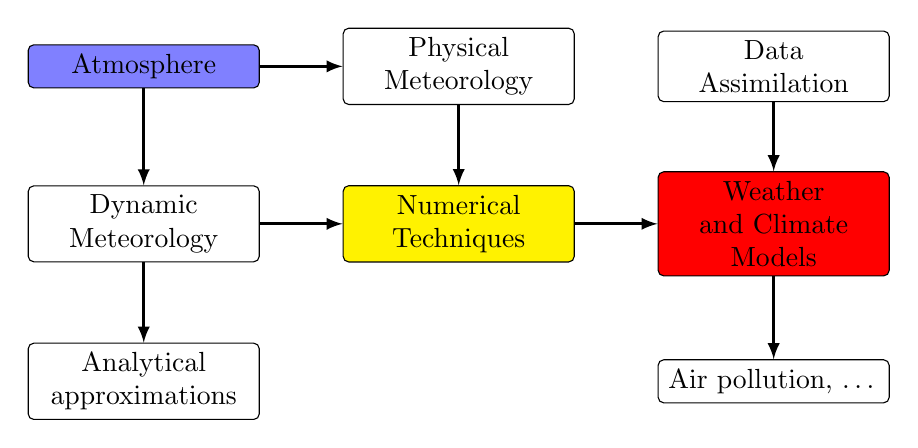
\begin{tikzpicture}
			\tikzstyle{every node}=[draw, text width=2.7cm, rounded corners=2pt,text centered]
			\node [fill=blue!50!] (atm) at (-4,2) {Atmosphere};
\uncover<2->{
			\node (dm) at (-4,0) {Dynamic\\ Meteorology};
			\node (pm) at (0,2) {Physical\\ Meteorology};
			\draw [-latex,line width=1pt] (atm) to (dm);
			\draw [-latex,line width=1pt] (atm) to (pm);
}
\uncover<3->{
			\node (anal) at (-4,-2) {Analytical\\ approximations};
			\node (da) at (4,2) {Data\\ Assimilation};
			\node [fill=yellow] (nt) at (0,0) {Numerical\\ Techniques};
			\node [fill=red] (nwp) at (4,0) {Weather\\ and Climate\\ Models};
			\node (ap) at (4,-2) {Air pollution, \ldots};
			\draw [-latex,line width=1pt] (dm) to (nt);
			%\draw [-latex,line width=1pt] (pm) to (nwp);
			\draw [-latex,line width=1pt] (da) to (nwp);
			\draw [-latex,line width=1pt] (nt) to (nwp);
			\draw [-latex,line width=1pt] (dm) to (anal);
			\draw [-latex,line width=1pt] (pm) to (nt);
			\draw [-latex,line width=1pt] (nwp) to (ap);
}
		\end{tikzpicture}
	\end{center}
	%
\end{frame}
%
%%%%%%%%%%%%%%%%%%%%%%%%%%%%%%%%%%%%%%%%%%%%%%%%%%%%%%%%%%%%%%%%%%%%%%
%
\begin{frame}
	\frametitle{Course objectives}
	%
	\begin{itemize}
		\item Get hold of problems that occur due to solving equations numerically (with a computer)\\[3ex]
\pause
		\item Distinguish these problems from other aspects of modeling
		\item Develop knowledge of existing solutions to these problems
		\item Be able to communicate with numerical analyst\\[3ex]
\pause
		\item Don't be frightened by code\\ \quad\ldots but it's no course on programming either!
	\end{itemize}
\end{frame}
%
%%%%%%%%%%%%%%%%%%%%%%%%%%%%%%%%%%%%%%%%%%%%%%%%%%%%%%%%%%%%%%%%%%%%%%
%
\begin{frame}
	\frametitle{Relation to AI-driven models}
	%
	\begin{itemize}
		\item AI-driven weather models are performing better and better, sometimes beating physics-based models on specific scores, often at a fraction of the computational cost\\[3ex]
		\item \emph{[personal assessment!]} This will make physics-based models less and less relevant, especially for operational weather forecasting\\[3ex]
		\item Nevertheless,\\[1ex]
		    \begin{itemize}
		        \item Physics-based models remain (for now) important for training AI models\\[1ex]
		        \item There is value in scientific understanding\\[1ex]
		        \item Many aspects treated in this course are also relevant for AI models, e.g. time-stepping, stability, scalability, etc.
		    \end{itemize}
	\end{itemize}
\end{frame}
%%
%%%%%%%%%%%%%%%%%%%%%%%%%%%%%%%%%%%%%%%%%%%%%%%%%%%%%%%%%%%%%%%%%%%%%%
%
\begin{frame}
	\frametitle{Course agenda}
	\vspace*{-5mm}
	\begin{center}
		\def\arraystretch{1.3}
		\begin{tabular}{l|lll}
			date	&	16h00	&	17h30 \\
		\hline
			22/09 	& Introduction,             &	(optional) Practicum	\\[-4pt]
					& Stability	                &   Python basics           \\
			29/09	& Time discretization		                            \\
			06/10	& Time discretization		&	Space discretization	\\[-4pt]
        			& (cont'd)					&	                    	\\
			13/10	& Space discretization		& 	Spectral methods        \\[-4pt]
					& (cont'd)					&	                 		\\
			27/10	& Nonlinearity      		&	Practicum				\\[-4pt]
					& 							&	Linux \& Fortran		\\
			10/11	& Semi-Implicit and		 	&	Project assignment		\\[-4pt]
					& Semi-Lagrangian models	&	+ finish practica       \\
		\hline
			17/11	& Parallel computing (TBC)  &	Project support session \\
			24/11	& Guest lecture (TBC)       &   Project support session	\\
			01/12	& Guest lecture (TBC)       &   Project support session	\\
			08/12	& Student project presentations
		\end{tabular}
		\def\arraystretch{1}
	\end{center}
\end{frame}
%
%%%%%%%%%%%%%%%%%%%%%%%%%%%%%%%%%%%%%%%%%%%%%%%%%%%%%%%%%%%%%%%%%%%%%%
%
\begin{frame}
	\frametitle{Course material}
	\vspace*{-5mm}
	\begin{itemize}
		\item Slides will appear on Ufora\vspace*{3ex}
		\item All material (slides sources, Jupyter notebooks) available on \texttt{https://github.com/ddegrauwe/ugent\_numtech}\vspace*{3ex}
		\item References:\vspace*{2ex}
			\begin{itemize}
				\item \emph{Numerical Methods for Wave Equations in Geophysical Fluid Dynamics},\\ Dale R. Durran, Springer, 1999, ISBN 0-387-98376-7.\vspace*{2ex}
				\item \emph{Chebyshev and Fourier Spectral Methods}, John P. Boyd, Springer, 2001, ISBN 978-3-540-51487-9.\vspace*{3ex}
			\end{itemize}
		\item Some papers (depending on project)
	\end{itemize}
\end{frame}
%
%%%%%%%%%%%%%%%%%%%%%%%%%%%%%%%%%%%%%%%%%%%%%%%%%%%%%%%%%%%%%%%%%%%%%%
%
\begin{frame}
	%
	\frametitle{Practical information}
	%
	\begin{itemize}
		\item (Check Ufora for modifications to time schedule)\vspace*{2ex}
		\item Practical sessions\vspace*{1ex}
			\begin{itemize}
				\item We will use High-Performance Computing (HPC) infrastructure of UGent: create account on\vspace*{1ex}
					\par
					\texttt{https://www.ugent.be/hpc/en/access/faq/access}\vspace*{1ex}
				\item access through browser via \texttt{https://login.hpc.ugent.be}\vspace*{1ex}
				\item \ldots or you can just install Linux on your laptop\vspace*{2ex}
			\end{itemize}
		\item Programs needed: python, Jupyter notebooks\vspace*{2ex}
		\item Evaluation: student project (2/3/4 persons) on simple model\vspace*{1ex}
			\begin{itemize}
				\item presentation for other students\vspace*{1ex}
				\item (small) report
			\end{itemize}
	\end{itemize}
\end{frame}
%
%%%%%%%%%%%%%%%%%%%%%%%%%%%%%%%%%%%%%%%%%%%%%%%%%%%%%%%%%%%%%%%%%%%%%%
%
\begin{frame}
	\begin{center}
		\usebeamercolor[fg]{frametitle}{%
			\LARGE%
			Questions?
		}
	\end{center}
\end{frame}
%
%%%%%%%%%%%%%%%%%%%%%%%%%%%%%%%%%%%%%%%%%%%%%%%%%%%%%%%%%%%%%%%%%%%%%%
%
\end{document}
%
